\documentclass[12pt,a4paper]{paper}
\usepackage[utf8]{inputenc}
\usepackage[english]{babel}
\usepackage{amsmath}
\usepackage{enumitem}
\usepackage{amsfonts}
\usepackage{amssymb}
\usepackage{amsmath}
\usepackage{tikz}
\usepackage{mathdots}
\usepackage{yhmath}
\usepackage{cancel}
\usepackage{color}
\usepackage{siunitx}
\usepackage{array}
\usepackage{multirow}
\usepackage{amssymb}
\usepackage{gensymb}
\usepackage{tabularx}
\usepackage{booktabs}
\usetikzlibrary{fadings}
\usepackage[left=2cm,right=2cm,top=2cm,bottom=2cm]{geometry}
\usepackage{Sweave}
\begin{document}
\title{STAT646 - Homework 5\\\small{Daniel Osorio - dcosorioh@tamu.edu\\Department of Veterinary Integrative Biosciences\\Texas A\&M University}}
\maketitle
\Sconcordance{concordance:Osorio_Daniel_HW5.tex:Osorio_Daniel_HW5.Rnw:%
1 22 1 1 0 15 1 1 2 1 0 2 1 3 0 1 2 6 1 1 2 1 0 1 1 3 0 1 2 2 1 1 16 15 %
0 1 6 5 0 1 3 2 0 1 9 11 0 1 2 6 1 1 2 1 0 1 1 1 4 3 0 1 12 11 0 1 11 %
13 0 1 2 6 1 1 2 1 0 1 2 5 0 1 2 2 1 1 6 11 0 1 2 4 1 1 2 1 0 2 1 3 0 1 %
2 5 1 1 4 3 0 1 1 3 0 1 2 3 1 1 2 1 0 5 1 4 0 1 2 2 1 1 2 1 0 1 1 8 0 2 %
1 4 0 1 2 11 1 1 2 1 0 1 1 1 2 1 0 4 1 4 0 1 2 1 3 8 0 1 2 3 1}

\begin{enumerate}
\item Consider a genome that consists of 1,000 bases. The genome is organized into 20 genes, each
of length 50 bases. The first 50 bases in the genome correspond to gene one, the next 50
bases to gene two, etc. In a particular sample containing mRNA transcripts from this genome,
suppose there are 25 mRNA copies of gene 5, 60 mRNA copies of gene 10, and 40 mRNA
copies of gene 15; none of the other genes are expressed. We apply NGS to create sequencing
reads of length 10 bases. We then align the reads back to the genome and use the resulting
read counts to quantify expression for each gene. Follow the instructions below to conduct a
simulation. For grading purposes, you need only provide your R code, the figure described in
part (e), and the read count table described in part (f).
\begin{enumerate}
\item Create the simulated genome by:
\begin{Schunk}
\begin{Sinput}
> set.seed(101)
> nt <- c("A", "C", "T", "G")
> genome <- paste(sample(nt, 1000, replace = TRUE), collapse = "")
\end{Sinput}
\end{Schunk}
\item Create the fragments to be sequenced. For transcript i, randomly pick a location in
the transcript at which to break. Once a break has been created, you have two smaller
fragments. If a fragment is less than our desired read length of 10, throw it away. If a
fragment is of length 10, 11, . . ., 14, its first 10 bases will be sequenced (so, it does not
need to be fragmented any further). If a fragment is of length 15 bases or greater, it will
be fragmented again. Repeat this sequence until you are left only with short (length $\in$
[10, 14]) fragments that are ready to be sequenced.
\begin{Schunk}
\begin{Sinput}
> genes <- unlist(strsplit(genome, split = "(?<=.{50})", perl = TRUE))
> mRNA <- c(rep(genes[5],25), rep(genes[10],60), rep(genes[15],40))
\end{Sinput}
\end{Schunk}
\item Create the sequenced reads. For fragment j, create a sequencing read by reading off
the genomic sequence corresponding to the first 10 bases of this fragment, allowing for
sequencing errors to occur in 5\% of all base calls.
\begin{Schunk}
\begin{Sinput}
> # Sequence break function
> breakFunction <- function(fragment){
+   out <- sapply(fragment, function(X){
+     if(nchar(X) >= 15){
+       X <- unlist(strsplit(X,""))
+       bPos <- sample(1:(length(X)-1),1)
+       out <- c(paste0(X[1:bPos], collapse = ""),
+                paste0(X[(bPos+1):length(X)], collapse = ""))
+       return(out)
+     } else {
+       return(X)
+     }})
+   out <- as.character(unlist(out))
+   return(out)
+ }
> # Fragments 
> jFragments <- unlist(sapply(mRNA, function(fragment){
+   while(any(nchar(fragment) >= 15)) {
+     fragment <- breakFunction(fragment)
+   }
+   return(fragment)},USE.NAMES = FALSE))
> # Filtering
> jFragments <- jFragments[nchar(jFragments) > 9 & 
+                            nchar(jFragments) < 15]
> # Adding errors and filtering first 10 nt
> jFragments <- sapply(jFragments, function(X){
+   X <- unlist(strsplit(X,""))
+   X <- X[1:10]
+   ntP <- rbinom(10, 1, prob = 0.05)
+   nNt <- sample(nt,sum(ntP))
+   X[ntP] <- nNt
+   X <- paste0(X,collapse = "")
+   return(X)},USE.NAMES = FALSE)
\end{Sinput}
\end{Schunk}
\item Align the reads to the genome. For this, use the pairwiseAlignment function from
Biostrings to do local alignment. Reward a base match with a score of +1, penalize a
base mismatch with a score of -1, and penalize a gap with a score of -10 (use gapOpening
= 0 and gapExtension = -10 in pairwiseAlignment). Use the randomization based test
to assign a p-value to the alignment of each read, and only keep the reads that align with
p-values < 0.05; to keep the computation time down, just do B = 100 randomizations,
instead of the B = 1,000 that we did in the classroom examples.
\begin{Schunk}
\begin{Sinput}
> library(Biostrings)
> library(pbapply)
> # Substitution matrix
> mat <- nucleotideSubstitutionMatrix(match = 1, 
+                                     mismatch = -1, 
+                                     baseOnly = TRUE)
> # P-Value Function
> pValueFun <- function(X,Score,B=100){
+   newSeq <- sapply(seq_len(B), function(Y){
+     paste0(sample(unlist(strsplit(X,""))),collapse = "")
+   })
+   bScores <- sapply(newSeq, function(X){
+     score(pairwiseAlignment(X,genome,type="local",
+                             substitutionMatrix=mat,
+                             gapOpening= 0, gapExtension = -10))
+   })
+   mean(bScores >= Score)
+ }
> # Making and filtering alignments
> alignments <- pblapply(jFragments, function(X){
+   o <- pairwiseAlignment(X,genome,type="local",
+                             substitutionMatrix=mat,
+                             gapOpening= 0, gapExtension = -10)
+   if(pValueFun(X,score(o)) < 0.05){
+     start <-o@subject@range@start
+     end <- (o@subject@range@start+o@subject@range@width)
+     return(start:end)
+   }
+ })
\end{Sinput}
\end{Schunk}
\item Tabulate the number of times each base in the genome was covered by one or more of
the aligned reads. Create a dot plot to visualize the coverages. By 'dot.plot', I just
mean a traditional dot plot in statistics not the specialized plot we made for comparing
two sequences. For example, suppose there are 14 reads that were aligned to overlap
with base k in the genome. Then, you would put 14 dots, one above the other, at the kth
location along the horizontal axis. Figure 1 on page 4 shows an example, for a scenario
in which there are just two genes.
\begin{Schunk}
\begin{Sinput}
> par(mar=c(2.5,2.5,1,1), mgp=c(1.5,0.5,0))
> plot(table(unlist(alignments)), xlim=c(1,1000), 
+      ylab="Coverage", ylim=c(0,60))
\end{Sinput}
\end{Schunk}
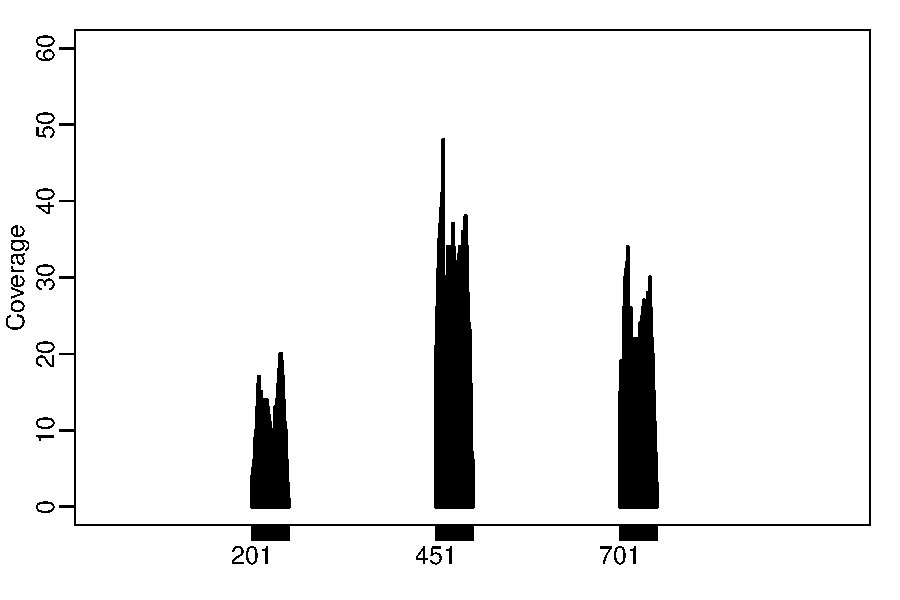
\includegraphics{Osorio_Daniel_HW5-005}
\item Tabulate the number of reads that overlapped, at least partially, with each of the three
expressed genes. For example, if 50 of the sequenced reads overlapped, at at least one
base, with gene 5, the read count for gene 5 would be 50.
\begin{Schunk}
\begin{Sinput}
> colSums(t(sapply(alignments, function(X){
+   c(any(X >= 201 & X <= 250),
+   any(X >= 451 & X <= 500),
+   any(X >= 701 & X <= 750))
+ })))
\end{Sinput}
\begin{Soutput}
[1]  57 147 104
\end{Soutput}
\end{Schunk}
\end{enumerate}
\item Context = “hammer” RNA-Seq data. These are read counts for ENSEMBL genes in rats
under two conditions: (1) spinal nerve ligation (SNL), which induces chronic neuropathic
pain, and (2) normal. We have four samples in each condition, two each at 2 weeks and 2
months after start (SNL was done at start in the SNL rats).
\begin{Schunk}
\begin{Sinput}
> library(DESeq2)
> hammerCounts <- read.table("hammer_counts.txt", header = TRUE, row.names = 1)
> hammerPhenoData <- read.table("hammer_phenodata.txt", header = TRUE)
\end{Sinput}
\end{Schunk}
\begin{center}
http://www.ncbi.nlm.nih.gov/pubmed?term=20452967
\end{center}
Use DESeq2 to analyze the data:
\begin{enumerate}
\item On the “rlog”-transformed counts:
\begin{Schunk}
\begin{Sinput}
> hammer <- DESeqDataSetFromMatrix(countData = hammerCounts,
+                                  colData = hammerPhenoData,
+                   design = ~protocol + Time + protocol:Time)
> rlogData <- rlog(hammer)
\end{Sinput}
\end{Schunk}
\begin{enumerate}
\item Carry out hierarchical clustering, using Euclidean distance and complete linkage.
Provide the resulting dendrogram and scree plots. How many clusters would you
say there are? Interpret the clusters with respect to the meta data. \textit{There are two clusters formed by the treatment and after that, each cluster is split into two subclusters by the covariate `time').}
\begin{Schunk}
\begin{Sinput}
> par(mfrow=c(1,2), mar=c(2.5,2.5,1,1),mgp=c(1.5,0.5,0))
> hCluster <- hclust(dist(t(assay(rlogData))))
> plot(hCluster$height)
> abline(h=35, col = "red", lty = 2)
> plot(hCluster)
> abline(h=35, col = "red", lty = 2)
\end{Sinput}
\end{Schunk}
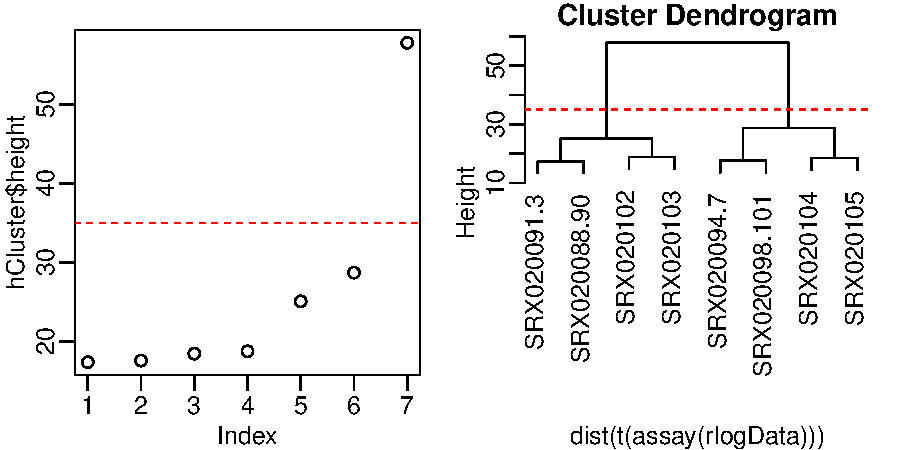
\includegraphics{Osorio_Daniel_HW5-009}
\item Carry out principal component analysis to explore structure among the rats(columns).
How much variation do the first two PCs account for? Interpret the eigenvectors
with respect to the meta data.\textit{The distribution of the points resemble the clusters produced by hierarchical clustering.}
\begin{Schunk}
\begin{Sinput}
> pComp <- prcomp(t(assay(rlogData)))
> summary(pComp)$importance[,1:2]
\end{Sinput}
\begin{Soutput}
                            PC1      PC2
Standard deviation     25.22689 10.07096
Proportion of Variance  0.74867  0.11932
Cumulative Proportion   0.74867  0.86799
\end{Soutput}
\begin{Sinput}
> par(mar=c(2.5,2.5,1,1),mgp=c(1.5,0.5,0))
> plot(pComp$x[,1:2])
\end{Sinput}
\end{Schunk}
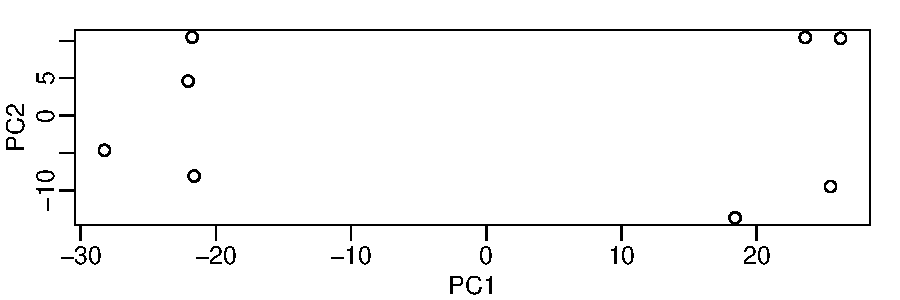
\includegraphics{Osorio_Daniel_HW5-010}
\end{enumerate}
\item As we have two factors (one each for treatment group (SNL vs. normal) and time (2
weeks vs. 2 months)), consider the following linear model for gene k’s counts:
\[E(Y_{ik}) = \beta_{ok} + \beta_{1k}Time_{i} + \beta_{2k}TX_{i}+\beta_{3k}(Time \times TX)_{i}\]
Where $Y_{ik}$ is the read count for gene $k$ in sample $i$, $Time_{i}$ is the indicator for whether sample $i$ was obtained at time 2 months (1 if yes, 0 if time 2 weeks), and $TX_{i}$ is the indicator for whether sample $i$ is from the treatment group (1 if yes, 0 if control). Under this model, there are separate means for each of the four comparisons group combinations; in other words, this model allows for an interaction between time and treatment.

For each gene, test for whether there is a treatment effect. Since there is an interaction, this translates to testing the null hypothesis that $\beta_{2k} = \beta_{3k} = 0$ for each $k = 1,2,\dots,m$ genes. This can be done via likelihood ratio test, comparing the `full' or `unrestricted' model from above to the `null' model:
\[E(Y_{ik} = \beta_{0k} + \beta_{1k}Time_{i}\]

The \texttt{DESeq2} package provides the function \texttt{nbinomLTR} for implementing a likelihood ratio test in the context of negative binomial regression. See its help file for details
\begin{enumerate}
\item Provide a histogram of the resulting p-values. Does the histogram look like you would it expect it to look? What does its shape tell you about whether or not there are differentially expressed genes? \textit{The high bar at the beginning of the plot means that there are several differentially expressed genes.}
\begin{Schunk}
\begin{Sinput}
> hammer <- estimateSizeFactors(hammer)
> hammer <- estimateDispersions(hammer)
> deHammer <- nbinomLRT(hammer, full = design(hammer), 
+                       reduced = ~ Time)
> deHammer <- results(deHammer,pAdjustMethod = "fdr")
> par(mar=c(2.5,2.5,1,1),mgp=c(1.5,0.5,0))
> hist(deHammer$pvalue, probability = TRUE)
> abline(v=0.05, col = "red", lty = 2, lwd=2)
\end{Sinput}
\end{Schunk}
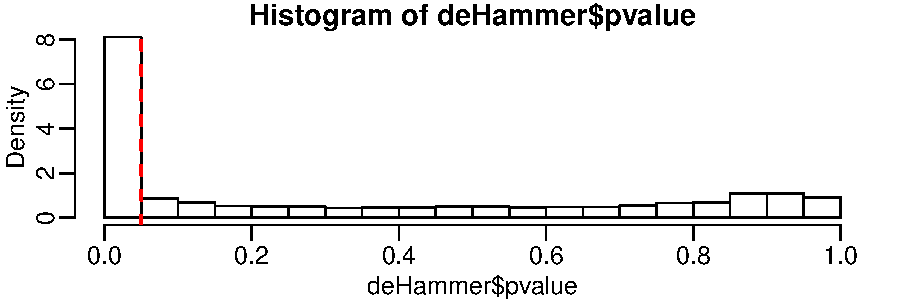
\includegraphics{Osorio_Daniel_HW5-011}
\item How many genes have absolute log2 fold change > 2 and FDR < 0.001? If out is the result of calling nbinomLRT, the log2 fold change values are in the column named “log2FoldChange” of results(out).
\begin{Schunk}
\begin{Sinput}
> sum(sapply(deHammer$log2FoldChange > 2, isTRUE) & 
+       sapply(deHammer$padj < 0.001, isTRUE))
\end{Sinput}
\begin{Soutput}
[1] 41
\end{Soutput}
\end{Schunk}
\end{enumerate}
\end{enumerate}
\end{enumerate}
\end{document}
